\section{Project Overview}
	In this product we want to recreate the old SNAKE game from the Nokia 3310 phone. The game will be created using an Nokia 5110 48 x 84 LCD matric display \cite{NokiaDisplay}; the same model that was used in the original Nokia 3310. The user will use a matrix keyboard to control the snake in the same way as in the original game. The system is driven by an ATMEGA 2560 that will read the user input, do the game calculations, and draw the game onto the display. In our version of snake, we are also keeping a highscore list. This highscore is saved in the non-volatile flash memory of the ATMEGA 2560 to ensure that it is persisted even if the power for the ATMEGA is off.

\section{System Description}
	In figure \ref{ProductComponents} the final result of the project can be seen. The red square shows the Arduino board containing the ATMEGA 2560 microcontroller. This is connected to the matrix keyboard highlighted in the blue square, and the Nokia display indicated with green. 
	
	\begin{figure}[H]
		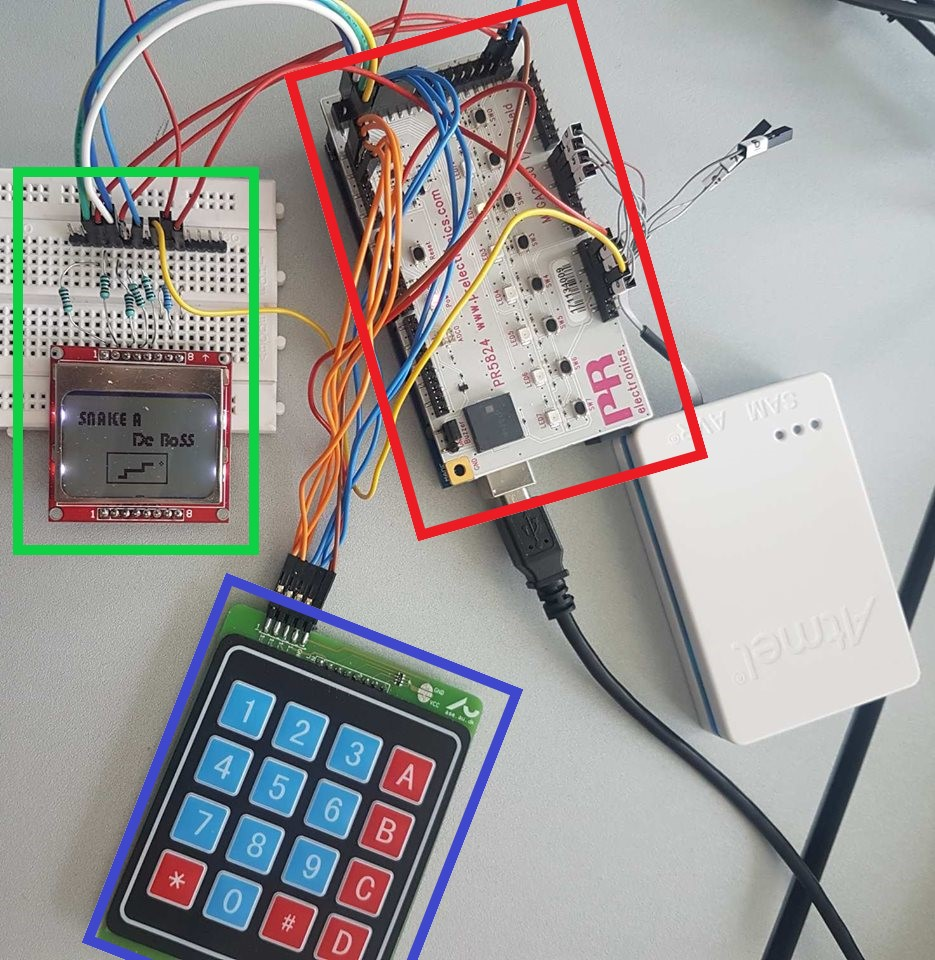
\includegraphics[width=12cm]{ProductComponents}
		\centering
		\caption{Picture of the setup}
		\label{ProductComponents}
	\end{figure}


	\subsection{Block Definition Diagram}
		Figure \ref{fig:bdd} gives an overview of the system from a hardware perspective. The block diagram shows the relations between the system's components and gives a general idea on how these components interact. The figure also includes a flow specification for SPI, since this connection is a non-atomic connection consisting of multiple signals. Table \ref{tb:blockDescriptions} following the diagram describes the blocks and their purpose.
		
		\begin{figure}[H]
			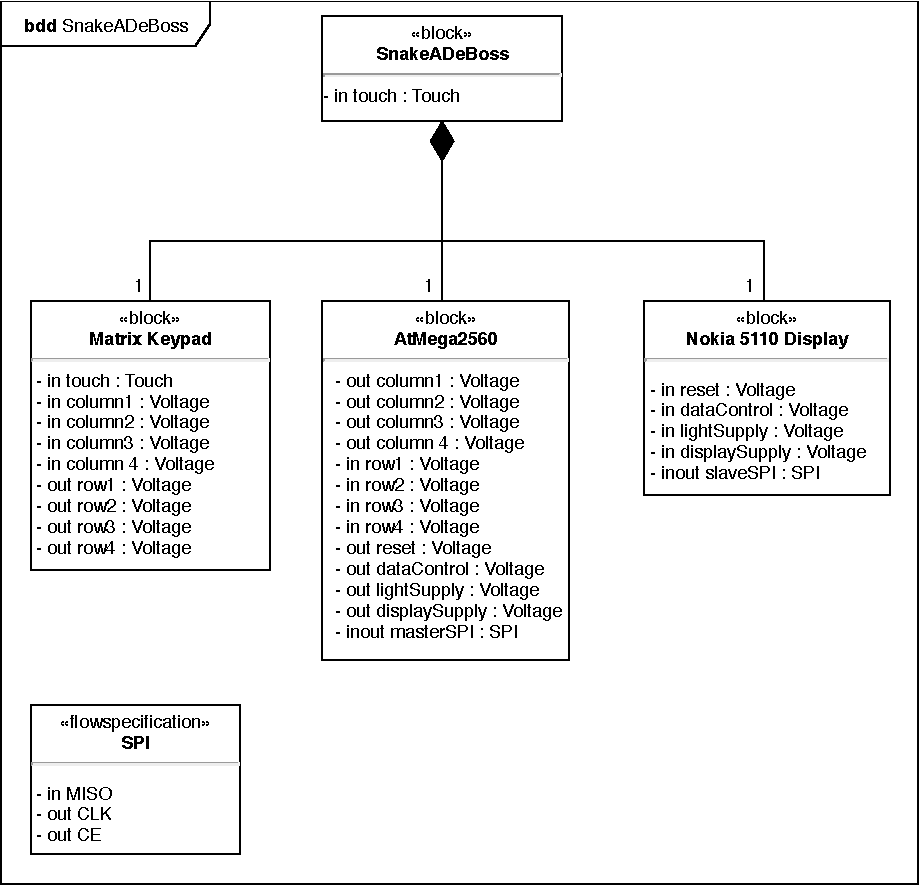
\includegraphics[width=14cm]{SnakeADeBossBDD}
			\centering
			\caption{BDD for SnakeADeBoss}
			\label{fig:bdd}
		\end{figure}
		
		\begin{table}[H]
			\centering
			\begin{tabular}{|l|l|}
				\hline
				\textbf{Block} & \textbf{Description} \\ \hline
				AtMega2560 & \begin{tabular}[c]{@{}l@{}}An AVR microcontroller. This component contains all game\\ logic and interfaces to Membrane Keyboard and Nokia 5110\\ Display.\end{tabular} \\ \hline
				Matrix Keyboard & \begin{tabular}[c]{@{}l@{}}A 4x4 membrane keypad. The user interacts with the system \\ via this component. The result of interactions with this com-\\ ponent is displayed on Nokia 5110 Display.\end{tabular} \\ \hline
				Nokia 5110 Display & \begin{tabular}[c]{@{}l@{}}A Nokia display. The user sees the game and scores on this\\ component.\end{tabular} \\ \hline
			\end{tabular}
			\caption{Block descriptions for SnakeADeBoss}
			\label{tb:blockDescriptions}
		\end{table}
		
		
	\subsection{Internal Block Diagram}
	\label{section:InternalBlockDiagram}
	
		Figure \ref{fig:ibd} shows the interal block diagram for SnakeADeBoss. This diagram describes the signals sent between the system's blocks. The tables following figure \ref{fig:ibd} describes the signals of the diagram.
		\begin{figure}[H]
			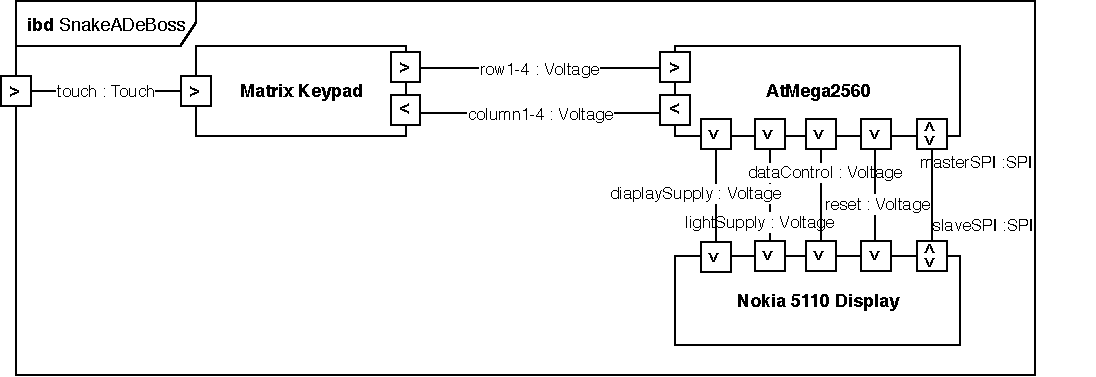
\includegraphics[width=14cm]{SnakeADeBossIBD}
			\centering
			\caption{IBD for SnakeADeBoss}
			\label{fig:ibd}
		\end{figure}
		
		\begin{table}[H]
			\centering
			\begin{tabular}{|l|l|l|l|}
				\hline
				\multicolumn{4}{|c|}{\textbf{Nokia 5110 Display}} \\ \hline
				Description & Signal & Direction & Signal Description \\ \hline
				\multirow{5}{*}{\begin{tabular}[c]{@{}l@{}}Display for gameplay. \\ Acts as a SPI slave during \\ SPI communication.\end{tabular}} & slaveSPI & IN/OUT & \begin{tabular}[c]{@{}l@{}}Type: SPI\\ Description: Dataconnection\\ between Nokia 5110 Display\\ and AtMega2560.\end{tabular} \\ \cline{2-4} 
				& reset & IN & \begin{tabular}[c]{@{}l@{}}Type: Voltage\\ Range: 0-3.3V\\ Description: Signal for reset\\ of the display.\end{tabular} \\ \cline{2-4} 
				& dataControl & IN & \begin{tabular}[c]{@{}l@{}}Type: Voltage\\ Range: 0-3.3V\\ Description: Signal indicating\\ data received in SPI bus is\\ command or data.\end{tabular} \\ \cline{2-4} 
				& displaySupply & IN & \begin{tabular}[c]{@{}l@{}}Type: Voltage\\ Range: 0-3.3V\\ Description: Power supply \\ for display.\end{tabular} \\ \cline{2-4} 
				& lightSupply &  & \begin{tabular}[c]{@{}l@{}}Type: Voltage\\ Range: 0-3.3V\\ Description: Power supply\\ for light on display.\end{tabular} \\ \hline
			\end{tabular}
			\caption{Signal description for Nokia 5110 Display}
			\label{tb:sigDisplay}
		\end{table}
				
		\begin{table}[H]
			\centering
			\begin{tabular}{|l|l|l|l|}
				\hline
				\multicolumn{4}{|c|}{\textbf{Matrix Keypad}} \\ \hline
				Description & Signal & Direction & Signal Description \\ \hline
				\multirow{3}{*}{\begin{tabular}[c]{@{}l@{}}User interacts with this\\ component to interact\\ with system.\end{tabular}} & touch & IN & \begin{tabular}[c]{@{}l@{}}Type: Touch\\ Description: Physical user-\\ input\end{tabular} \\ \cline{2-4} 
				& row1-4 & OUT & \begin{tabular}[c]{@{}l@{}}Type: Voltage\\ Range: 0-3.3V\\ Description: Signal for row on\\ Keypad.\end{tabular} \\ \cline{2-4} 
				& column1-4 & IN & \begin{tabular}[c]{@{}l@{}}Type: Voltage\\ Range: 0-3.3V\\ Description:  Signal for row on\\ Keypad.\end{tabular} \\ \hline
			\end{tabular}
			\caption{Signal description for Matrix keypad}
			\label{table:MembraneKeypad}
		\end{table}
		
		\begin{table}[H]
			\centering
			\begin{tabular}{|l|l|l|l|}
				\hline
				\multicolumn{4}{|c|}{\textbf{AtMega2560}} \\ \hline
				Description & Signal & Direction & Signal Description \\ \hline
				\multirow{7}{*}{\begin{tabular}[c]{@{}l@{}}This component contains \\ display logic for Nokia\\ 5110 Display and handles \\ input from Membrane \\ Keypad\end{tabular}} & masterSPI & IN/OUT & \begin{tabular}[c]{@{}l@{}}Type: SPI\\ Description: Dataconnection\\ between AtMega2560\\ and Nokia 5110 Display.\end{tabular} \\ \cline{2-4} 
				& reset & OUT & \begin{tabular}[c]{@{}l@{}}Type: Voltage\\ Range: 0-3.3V\\ Description: Signal for reset\\ of the display.\end{tabular} \\ \cline{2-4} 
				& dataControl & OUT & \begin{tabular}[c]{@{}l@{}}Type: Voltage\\ Range: 0-3.3V\\ Description: Signal indicating\\ data received in SPI bus is\\ command or data.\end{tabular} \\ \cline{2-4} 
				& displaySupply & OUT & \begin{tabular}[c]{@{}l@{}}Type: Voltage\\ Range: 0-3.3V\\ Description: Power supply \\ for display.\end{tabular} \\ \cline{2-4} 
				& lightSupply & OUT & \begin{tabular}[c]{@{}l@{}}Type: Voltage\\ Range: 0-3.3V\\ Description: Power supply\\ for light on display.\end{tabular} \\ \cline{2-4} 
				& row1-4 & IN & \begin{tabular}[c]{@{}l@{}}Type: Voltage\\ Range: 0-3.3V\\ Description: Signal for row \\ on keypad.\end{tabular} \\ \cline{2-4} 
				& column1-4 & OUT & \begin{tabular}[c]{@{}l@{}}Type: Voltage\\ Range: 0-3.3V\\ Description: Signal for \\ column on keypad.\end{tabular} \\ \hline
			\end{tabular}
			\caption{Signal description for AtMega2560 Keypad}
			\label{}
		\end{table}
